\documentclass[12pt]{article}
\usepackage{/home/pacman/Documents/tex-packages/NotesTeXV3}
%\usepackage{marginnote, sidenotes, fancyhdr, titlesec, geometry, tcolorbox}
%/Path/to/package should be replaced with package location
\usepackage{bbold}
\usepackage{cancel}
\usepackage{tabularx}
\hypersetup{
    colorlinks,
    citecolor=black,
    filecolor=black,
    linkcolor=red,
    urlcolor=red
}


\title{{\Huge Lectures on Quantum Mechanics}\\{\Large{SEM02-2023}}}
\author{Gabriel Balarezo\footnote{\href{https://google.com/}{\textit{https://github.com/GabrielBJ}}}}

\affiliation{Yachay Tech University \\ School of Nanotechnology and Physical Sciences \\ Urcuqui, Ecuador}
\emailAdd{balarezog961@gmail.com}
\begin{document}
  \maketitle
  \flushbottom
  \newpage
  \pagestyle{fancynotes}
  \part*{Introduction}
Quantum mechanics is certainly the most successful theory of the physical world at small scales. It is also one of the most mysterious.
  
  Some notes here.
\newpage
  \part{Time Independent Non-degenerate Perturbation Theory}

  \section{Lecture 1}
%%%%%%%%%%%%%%%%%%%%%%%%%%%%%%%%%%%%%%%%%%%%%%%%%%%%%%%%%%%%%%%%%%%%%%%%%%%%%%%%%%%%%%%%%%%%%%%%%%%
%%%%%%%%%%%%%%%%%%%%%%%%%%%%%%%%%%%%%%%%%%%%%%%%%%%%%%%%%%%%%%%%%%%%%%%%%%%%%%%%%%%%%%%%%%%%%%%%%%%
%%%%%%%%%%%%%%%%%%%%%%%%%%%%%%%%%%%%%%%%%%%%%%%%%%%%%%%%%%%%%%%%%%%%%%%%%%%%%%%%%%%%%%%%%%%%%%%%%%%
Suppose we have a "known" system with Hamiltonian, eigenfunctions and eigenenergies $\displaystyle{H_0}$,  $\displaystyle{\Psi_n}$ and $\displaystyle{E_n}$ respectively.
  \begin{equation*}
    \hat{H} |\Psi_n \rangle = E_n |\Psi_n \rangle 
\end{equation*}
where
\sn{The student may remember the Kronecker delta from his/her Quantum Mechanics I course.}
$$\langle \hat{\Psi} |\hat{H}|\hat{\Psi} \rangle = E_n,\,\,\,\,\,\,\,\,
	\langle \Psi_n | \Psi_{n'} \rangle = \delta_{nn'} $$
So that $\{\displaystyle{\Psi_n}\}$ forms a orthonormal basis over the Hilbert space of $\displaystyle{H_0}$. 
We apply a perturbative potential $\tilde{V}$ \sn{$\tilde{V}$ is very small compared to $H_0$.} to $H_0$, yielding a new Hamiltonian. 
for the perturbated system,
\begin{equation}
\label{eq:1}
  \tilde{H} = \hat{H_0} + \lambda \tilde{V},\,\,\,\,\text{let}\,\,\lambda \in [0,1]
\end{equation}
a "bookkeeping parameter" to keep track of the relative signs of from in order of the perturbated 
potential.
\subsection{Method}
Express the wave functions and eigenenergies of the perturbated Hamiltonian $H$, $\tilde{\psi}$, $\tilde{E}_n$ 
as a power series equation in orders of $\lambda$.
\begin{align*}
	\tilde{E}_n & = \tilde{E}^{(0)}_0 + \lambda \tilde{E}^{(1)}_n + \lambda^2 \tilde{E}^{(2)}_n
	+ \cdots = \sum_{k} \lambda^{k} \tilde{E}^{(k)}_n\\
	\tilde{\psi}_n & = \tilde{\psi}^{(0)}_n + \lambda \tilde{\psi}^{(1)}_n + \lambda^2 \tilde{\psi}^{(2)}_n 
	+ \cdots = \sum_{k} \lambda^k \tilde{\psi}^{(k)}_n
\end{align*}
Now we write the Time independent Schr\"odinger equation for the perturbated Hamiltonian,
\begin{align}
  \tilde{H} \big|\tilde{\psi}_n \big > & = \tilde{E}_n \big|\tilde{\psi}_n \big >\\
	(\hat{H} + \hat{V}) \sum_{k} \lambda^k \big| \psi^{(k)}_n \big > & = \sum_{k} \lambda^k \tilde{E}^{(k)}_n \sum_{k}
	\lambda^k \big|\psi^{(k)}_n \big>\\
	\sum_{k}(\lambda^k \hat{H}_0 + \lambda^{k+1} \hat{V}) \big|\hat{\psi}^{(k)}_n \big > & = \sum_{k'} \sum_{k}
	\lambda^{k'+k} \hat{E}^{(k)}_n \big| \hat{\psi}^{(k)}_n \big >
\end{align}
\begin{equation}
	\sum_{k} \left(\lambda^k \hat{H}_0 + \lambda^{k+1} \hat{V} - \sum_{k'} \lambda^{k'+ k}  
	\hat{E}^{(k')}_n \right ) \big|\psi^{(k)}_n \big > = 0 
\end{equation}
\begin{equation}
  \label{eq:6}
	\sum_{k} \lambda^{k} \left(\hat{H}_0 \big| \hat{\psi}^{(k)}_n \big > + \underbrace{(1 - \delta_
	{k0})}_{k\neq 0} \hat{V} \big| \hat{\psi}^{(k-1)} \big > - \sum_{k=0}^{k} \hat{E}^{(k')}_n 
	\big | \hat{\psi}^{(k-k')}_n \big > \right ) = 0
\end{equation}
Since Equation \ref{eq:6} is true for any value of $\lambda$, it must hold for each power of $\lambda$ separately:
\begin{align*}
	\mathcal{O}(1)_{k=0} & = \hat{H} \big | \hat{\psi}^{(0)}_n \big > + (1 - \delta_{k0}) \hat{V}
	\big | \hat{\psi}^{(-1)}_n \big >\\
	& = \sum_{k' = 0}^{0} \hat{E}^{(k')}_n \big| \hat{\psi}^{(0-k')}_n \big>\\
	\Longrightarrow \hat{H}_0 \big| \hat{\psi}^{(0)}_n \big > & = \hat{E}^{(0)}_n \big| \hat{\psi}^{(0)}_n \big>\\
  \big < \psi_n \big | \underbrace{H_0}_{\mathclap{\text{hermitian}}} \big| \hat{\psi}^{(0)}_n \big > & = \hat{E}^{(0)}_n \big < \psi_n   \big |
	\hat{\psi}^{(0)}_n\big>
\end{align*}
\begin{equation*}
  \big < \psi_{n'} \big|\hat{H}_0 ^\dag = E_{n'} \big < \psi_{n'} \big |
\end{equation*}
\begin{equation*}
	(E_{n'} - \hat{E}^{(0)}_n)\big < \psi_{n'} \big|\hat{\psi}^{(0)}_n \big > = 0
\end{equation*}
So,
\begin{equation}
  \hat{E}^{(0)}_n = E_n\,\,\,\text{or}\,\,\,\big < \psi_n \big| \hat{\psi}^{(0)}_n \big > = 0 
\end{equation}
\noindent
If the system $\hat{H}_0$ is nondegenerate: 
\[ \Longrightarrow \big|\hat{\psi}^{(0)}_n\big> = \big| \psi_n \big >\]
If the system is degenerate, then:
\begin{equation*}
	\hat{H}_0 \big|\psi_{n'} \big > = E_n \big| \psi_{n'} \big >\,\,\,\,\text{for } n' \in \{n, \cdots, n+k\}
\end{equation*}
Then:
\begin{equation*}
	\big | \hat{\psi}^{(0)}_n \big > = \sum_{k'=0}^{k} C_{n+k'} \big|\psi_{n+k'} \big >
\end{equation*}
\begin{equation*}
	\hat{E}_n = E_n \mathcal{O}(\lambda)
\end{equation*}
\begin{equation*}
	\big | \hat{\psi}_n \big > = | \psi_n\big > + \mathcal{O}(\lambda)
\end{equation*}
\begin{equation*}
\mathcal{O}(\lambda): \hat{H}_0 \big|\hat{\psi}^{(1)}_n \big> + \hat{V} \big|\hat{\psi}^{(0)}_n \big>
= E_n^{(0)} \big|\hat{\psi}^{(1)}_n \big> + \hat{E}^{(1)}_n  \big|\hat{\psi}^{(0)}_n \big> 
\end{equation*}
multiply by $\big<\psi_{n'} \big|$:
\begin{equation*}
\big<\psi_{n'} \big|\hat{H}_0 \big|\hat{\psi}^{(1)}_n \big> + \big<\psi_{n'} \big|\hat{V} \big|\hat{\psi}^{(0)}_n \big>
= E_n^{(0)}\big<\psi_{n'}\big|\hat{\psi}^{(1)}_n \big> + \hat{E}^{(1)}_n \big<\psi_{n'} \big|\hat{\psi}^{(0)}_n \big> 
\end{equation*}
\begin{equation*}
	\big<\psi_{n'} \big|\hat{H}_0 = E_{n'} \big<\psi_{n'} \big|
\end{equation*}
$$
\big|\hat{\psi}^{(0)}_n \big> = \big|\psi_n \big>\,\,\,\,\text{(non-degenerate)},\,\,\,\hat{E}^{(0)}_n = E_n
$$
\begin{equation}
	(E_{n'}-E_n)\big< \psi_{n'} \big|\hat{\psi}^{(1)}_n \big> + \big < \psi_{n'} \big| \hat{V}\big|\psi_n \big>
	= \hat{E}^{(1)}_n \delta_{n'n}
\end{equation}
\textbf{if} $\mathbf{n'= n}$:
\begin{equation*}
	\cancelto{0}{(E_{n'}-E_n)} \big< \psi_{n'} \big|\hat{\psi}^{(1)}_n \big> + \big < \psi_{n'} \big| \hat{V}\big|\psi_n \big>
	= \hat{E}^{(1)}_n \delta_{n'n}
\end{equation*}
\begin{align}
	\Longrightarrow \hat{E}^{(1)}_n & = \big < \psi_{n} \big| \hat{V}\big|\hat{\psi}^{(1)}_n \big>\nonumber\\
	\hat{E}_n & = E_n + \big < \psi_{n'} \big| \hat{V}\big|\hat{\psi}^{(1)}_n \big> + \mathcal{O}(\lambda^2)\nonumber\\
	\big | \hat{\psi}_n \big > & = \big| \psi_n \big> + \mathcal{O} (\lambda)
\end{align}
\textbf{if} $\mathbf{n'\neq n}$:
\begin{equation*}
	(E_{n'}-E_n)\big< \psi_{n'} \big|\hat{\psi}^{(1)}_n \big> = -\big < \psi_{n'} \big| \hat{V}\big|\psi_n \big>
	+ \hat{E}^{(1)}_n \cancelto{0}{\delta_{n'n}}
\end{equation*}
\begin{equation}
	\big< \psi_{n'} \big|\hat{\psi}^{(1)}_n \big> = \frac{\big < \psi_{n'} \big| \hat{V}\big|\psi_n \big>}{E_n - E_{n'}}
\end{equation}
Since $\{ \psi_n\}$ forms an orthonormal basis,
\begin{equation*}
	\Longrightarrow \sum_{n'} \big|\psi_{n'} \big> \big< \psi_{n'} \big | = \mathbb{1}\,\,\,\text{Identity matrix}
\end{equation*}
\begin{align}
	\big| \hat{\psi}^{(1)}_n \big > = \mathbb{1} \big|\hat{\psi}^{(1)}_n\big> & = \sum_{n'} \big|\psi_{n'}
	\big> \big < \psi_{n'} | \hat{\psi}^{(1)}_n \big>\nonumber\\
	& = \sum_{n'=n} \frac{\big < \psi_{n'} \big| \hat{V}\big|\psi_n \big>}{E_n- E_{n'}} \big|\psi_{n'} \big> 
\end{align}
Since $\big |\hat{\psi}^{(0)}_n \big> = \big| \psi_{n} \big>$, then $\big |\hat{\psi}^{(1)}_n \big>$
cannot depend on $\big|\psi_n\big>$. 
\newpage
%%%%%%%%%%%%%%%%%%%%%%%%%%%%%%%%%%%%%%%%%%%%%%%%%%%%%%%%%%%%%%%%%%%%%%%%%%%%%%%%%%%%%%%%%%%%%%%%%%%
%%%%%%%%%%%%%%%%%%%%%%%%%%%%%%%%%%%%%%%%%%%%%%%%%%%%%%%%%%%%%%%%%%%%%%%%%%%%%%%%%%%%%%%%%%%%%%%%%%%
%%%%%%%%%%%%%%%%%%%%%%%%%%%%%%%%%%%%%%%%%%%%%%%%%%%%%%%%%%%%%%%%%%%%%%%%%%%%%%%%%%%%%%%%%%%%%%%%%%%
\section{Lecture 2}
In the previous lecture we defined the perturbed hamiltonian
\sn{$\tilde{H}$: perturbed hamiltonian, $\hat{H}_0$: unperturbed hamiltonian, $\lambda$: bookkeeping parameter,\\ $\hat{V}$: perturbing potential.}
(Equation \ref{eq:1}) as:
\begin{equation*}
  \tilde{H} = \hat{H}_0 + \lambda \hat{V}
\end{equation*}
\noindent
$\hat{V}$ needs to be smaller than $\hat{H}_0$, $\lambda$ keeps track of this, i.e., dependence on $\hat{V}$.
Writing the Schr\"odinger equation:
\begin{equation*}
	(\hat{H}_o + \lambda \hat{V}) \hat{\psi}_n = \tilde{E}_n \tilde{\psi}_n
\end{equation*}
$\tilde{E}_n$ and $\tilde{\psi}_n$ are eigenenergies and wavefunctions for the perturbated hamiltonian.

Expand $\tilde{E}_n$ and $\tilde{\psi}_n$ in power of $\lambda$
\begin{align*}
	\tilde{E}_n & = \hat{E}^{(0)}_n + \lambda \tilde{E}^{(1)}_n + \lambda^2 \tilde{E}^{(2)}_n + \mathcal{O}(\lambda^3)\\
	\tilde{\psi}_n & = \hat{\psi}^{(0)}_n + \lambda \tilde{\psi}^{(1)}_n + \lambda^2 \tilde{\psi}^{(2)}_n + \mathcal{O}(\lambda^3)
\end{align*}
and substitute for $\tilde{E}_0$ and $\tilde{\psi}_n$ into the (SE) and collect terms of like powers of $\lambda$.
\begin{equation*}
	\mathcal{O}(1): \hat{H}_0 \big|\tilde{\psi}^{(0)}_n \big> = \tilde{E}^{(0)}_0 \big| \psi_n^{(0)} \big>
\end{equation*}
Multiply by $\big< \psi_{n'}\big|$,
\begin{equation*}
	\big< \psi_{n'}\big|\hat{H}_0 \big|\tilde{\psi}^{(0)}_n \big> = \tilde{E}^{(0)}_0 \big< \psi_{n'}\big| \psi_n^{(0)} \big>
\end{equation*}
since $\hat{H}_0 = H_0^\dag$ since $\hat{H}_0$ is hermitian
\begin{equation*}
	\big < \psi_{n'} \big| \hat{H}^\dag_0 = E_{n'} \big< \psi_{n'} \big|\,\,\,\text{(SE) for } \hat{H}_0
\end{equation*}
\begin{equation*}
	\Longrightarrow E_{n'} \big< \psi_{n'} \big| \psi_n^{(0)} \big> = 
	\hat{E}^{(0)}_0\big< \psi_{n'} \big| \psi_n^{(0)} \big> 
\end{equation*}
$$E^{(0)}_{n'} = E_{n'}\,\,\,\,\text{or}\,\,\,\,\big< \psi_{n'} \big| \psi_n^{(0)} \big> = 0$$

$\tilde{\psi}_n^{(0)} = \sum_{n'} \big< \psi_{n'} \big| \psi_n^{(1)} \big> $
\\
\\
If $E_n$ is k-level degenerate, then
\begin{equation}
	\big| \tilde{\psi}^{(0)}_n \big> = \sum_{n'=n}^{n+k-1} \big< \psi_{n'} \big| \psi_n^{(0)} \big>
	\big|\psi_{n'} \big>
\end{equation}

Consider $\hat{H}_0$ to be non-degenerate 
$$
	\Longrightarrow E^{(0)}_n = E_n,\,\,\,\,\big|\big< \psi_n | \tilde{\psi}^{(0)}_n \big> \big| ^2 = 0
$$
$$\sum_{n'=n}^{n+k-1}\big| \big< \psi_{n'} \big| \psi_n^{(0)} \big> \big|^2 = 1$$
since $ \big< \psi_{n'} \big| \psi_n^{(0)} \big> = 0\,\,\text{for }n'\neq n$,
$$\Longrightarrow \big| \tilde{\psi}^{(0)}_n \big > = \big| \psi_{n'} \big>$$
the $n^{th}$ eigenenergy of the perturbated system (hamiltonian) $\tilde{E}_n$ is the $n^{th}$ 
eigenenergy of the unperturbed system to Zeroth order in the perturbation, i.e $\mathcal{O}(\lambda^0)
= \mathcal{O}(1),\,\,\lambda = 0 $.

If we turn the perturbation off we get the eigenenergy of the unperturbed system
$\because$ the $n^{th}$ wavefunction for the perturbed hamiltonian $\tilde{\Psi}_n$ is a linear 
combination of the unperturbed hamiltonian's degenerate wavefunctions with energy $E_n$ to Zeroth
order in the perturbation, i.e $\mathcal{O}(\lambda^0) = \mathcal{O}(1)\,\,\,\text{or}\,\,\,\lambda = 0$ 
\begin{equation*}
	\Longrightarrow \big|\hat{\psi}^{(0)}_n \big> =\sum_{n'=n}^{n+k-1}
	\big< \psi_{n'} \big|\tilde{ \psi}_n^{(0)} \big> \big|\psi_{n'}\big>
\end{equation*}
,where
$$\sum_{n'=n}^{n+k-1}\big| \big< \psi_{n'} \big| \tilde{\psi}_n^{(0)} \big> \big|^2 = 1$$

Even if we "turn off" the perturbation, it can still left the degeneracy of $\{\big|\psi_n\big>,
\cdots, \big|\psi_{n+k-1}\big>\}$ for k-fold degenerate systems, unless the unperturbed wavefunctions
are eigenstates of the perturbation.\\

Now let's assume $\hat{H}_0$ is non-degenerate
$$\Longrightarrow \big| \big< \psi_{n'} \big| \tilde{\psi}_n^{(0)} \big> \big|^2 = 1$$
wlog $\psi_n = \tilde{\psi}^{(0)}_n$ (Choice of 1 for phase factor),
\begin{align*}
	\tilde{E}_n & = E_n + \mathcal{O}(\lambda)\\
	\tilde{\psi}_n & = \psi_n + \mathcal{O}(\lambda)
\end{align*}
and gather together terms of order 1 in $\lambda$ in the (SE)
\begin{equation}
	\mathcal{O}(\lambda):\lambda \left( \hat{H}_0 \big|\tilde{\psi}^{(1)}_n \big> + 
	\hat{V}\big| \tilde{\psi}^{(0)}_n\big> \right) = 
	\lambda \left(E_n \big|\tilde{\psi}^{(1)}_n \big> + E^{(1)}_n \big|\psi_n \big> \right)
\end{equation}
setting $\lambda = 1$,

\begin{equation}
  \label{eq:2.3}
	\hat{H}_0 \big|\tilde{\psi}^{(1)}_n \big> + 
	\hat{V}\big| \tilde{\psi}^{(0)}_n \big> = 
	E_n \big|\tilde{\psi}^{(1)}_n \big> + E^{(1)}_n \big|\psi_n \big> 
\end{equation}
\marginnote{\fontsize{10}{4}\selectfont
  \emph{Equation \ref{eq:2.3} is a recursive equation relating the 1st order corrections in $\tilde{E}_n$ and $\tilde{\psi}_n$
to the Zeroth order corrections, in the unperturbed eigenenergy and wavefunction, $E_n$ and $\psi_n$
respectively $\because$ the $\mathcal{O}^{th}$ relates the kth order corrections to all previous orders.}
  }
%%%%%%%%%%%%%%%%%%%%%%%%%%%%%%%%%%%%%%%%%%%%%%%%%%%%%%%%%%%%%%%%%%%%%%%%%%%%%%%%%%%%%%%%%%%%%%%%%%%
%%%%%%%%%%%%%%%%%%%%%%%%%%%%%%%%%%%%%%%%%%%%%%%%%%%%%%%%%%%%%%%%%%%%%%%%%%%%%%%%%%%%%%%%%%%%%%%%%%%
%%%%%%%%%%%%%%%%%%%%%%%%%%%%%%%%%%%%%%%%%%%%%%%%%%%%%%%%%%%%%%%%%%%%%%%%%%%%%%%%%%%%%%%%%%%%%%%%%%%
\subsection{Two Unknowns}

Use the fact that
\[\big< \psi_{n'} \big| \psi_n\big> = \delta_{n'n}\,\,\,\,\text{and}\,\,\,\,\hat{H}_o \big|\psi_{n'}
\big> = E_{n'} \big | \psi_{n'} \big>\]
to obtain equations for $\tilde{E}^{(1)}_n$ and $\tilde{\psi}^{(1)}_n$.\\

Multiply by $\big< \psi_{n'} \big|$ 
\begin{equation*}
	\big< \psi_{n'} \big|\hat{H}^\dag_o \big|\tilde{\psi}^{(1)}_n \big> + 
	\big< \psi_{n'} \big|\hat{V}\big| \tilde{\psi}^{(0)}_n \big> = 
	E_n \big< \psi_{n'} \big|\tilde{\psi}^{(1)}_n \big> + E^{(1)}_n \underbrace{\big< \psi_{n'}
	\big|\psi_n \big>}_{\delta_{n'n}} 
\end{equation*}
\begin{equation}
\label{eq:2.4}
	\left(E_{n'} - E_n\right)\big< \psi_{n'} \big|\tilde{\psi}^{(1)}_n \big> +
	\big< \psi_{n'} \big|\hat{V}\big| \psi_n \big> = \tilde{E}^{(1)}_n \delta_{n'n}
\end{equation}
$\big< \psi_{n'} \big|\tilde{\psi}^{(1)}_n \big>  $ is the coefficient of $\big|\psi_{n'} \big>$.\\
\\
$\tilde{E}^{(1)}_n $: First order correction to the eigenenergy.\\

If $n'=n$, Equation \ref{eq:2.4} yields to $\tilde{E}^{{(1)}}_n$ 
\begin{equation*}
	\boxed{\tilde{E}^{(1)}_n =	\big< \psi_{n} \big|\hat{V}\big| \psi_n \big>  }
\end{equation*}
which is the expectation value of the perturbation in the $n^{th}$ eigenstate of the unperturbed hamiltonian.
\\

On the other hand, if $n'\neq n$, Equation \ref{eq:2.4} yields to coefficients of $\big | \tilde{\psi}^{(1)}_n\big>$ and $\lambda = 1$.
\begin{equation*}
	\big < \psi_{n'} |\hat{\psi}^{(1)}_n \big> = \frac{\big< \psi_{n'}\big|\hat{V}\big|\psi_n
	\big>}{E_n - E_{n'}}
\end{equation*}
\begin{equation*}
	\big|\tilde{\psi}^{(1)}_n \big> = \sum_{n' \neq n}
	\frac{\big< \psi_{n'}\big|\hat{V}\big|\psi_n\big>}{E_n - E_{n'}}\big|\psi_{n'}\big>
\end{equation*}
\begin{equation*}
	\tilde{E}_n = E_n +\big< \psi_{n}\big|\hat{V}\big|\psi_n\big> + \mathcal{O}(\lambda^2) 
\end{equation*}
\begin{equation}
	\big| \tilde{\psi}_n \big> = \big| \psi_n \big> +\sum_{n' \neq n}
	\frac{\big< \psi_{n'}\big|\hat{V}\big|\psi_n\big>}{E_n - E_{n'}}\big|\psi_{n'}\big> + \mathcal{O}(\lambda^2)
\end{equation}

The first order correction to the eigenenergy is the energy of the perturbation if you stay in the
$n^{th}$ eigenstate of the unperturbed system. So $V$ \sn{\textbf{Note:} if $\hat{V}$ (the perturbation) is an odd function:
\begin{align*}
  \hat{E}^{(1)}_n &= \int d^3 \vec{r}\big|\underbrace{\psi(\vec{r})}_\text{even}
	\big|^2 \overbrace{\hat{V}(\vec{r}, t)}^\text{odd}\\
  &= 0
\end{align*}} has to be "weak" so that you can remain in
$\big|\psi_n\big>$ under its action.

The first order corrections to wavefunctions are proportional to the matrix elements of  
$$\big<\psi_{n'}\big|\hat{V}\big|\psi_n\big>,$$
i.e., that under the action of the perturbation you can transition from $n^{th}$ to $n^{'th}$ 
eigenstate of the unperturbed hamiltonian and inversely proportional to the difference (energy)
between the eigenenergies of the $n^{th}$ and $n^{'th}$  eigenstates of the perturbed hamiltonian.
\marginnote{\fontsize{10}{4}\selectfont
 \textbf{Note:}
\begin{equation*}
	\big|\big<\psi_{n'} \big| \hat{V}\big| \psi_n \big> \big| \ll \big|E_n - E_{n'}\big|
\end{equation*}
\emph{
Otherwise our expression for the wavefunctions of the perturbed system won't converge.
  }}

Setting  $$\lambda \gg 1$$
\begin{equation*}
	\mathcal{O}(\lambda ^2): \hat{H}_o \big|\tilde{\psi}^{(2)}_n\big> + \hat{V}\big|\tilde{\psi}^{(1)}_n\big>
	= E_n \big|\tilde{\psi}^{(2)}_n \big> + \tilde{E}^{(1)}_n \big|\tilde{\psi}^{(1)}_n \big>
	+ \tilde{E}^{(2)}_n \big| \psi_n \big>
\end{equation*}
and multiplying by $\big< \psi_{n'} \big|$
\begin{equation*}
	\big< \psi_{n'} \big|\hat{H}_o \big|\tilde{\psi}^{(2)}_n\big> + 
	\big< \psi_{n'} \big|\hat{V}\big|\tilde{\psi}^{(1)}_n\big>
	= E_n \big< \psi_{n'} \big|\tilde{\psi}^{(2)}_n \big> + 
	\tilde{E}^{(1)}_n \big< \psi_{n'} \big|\tilde{\psi}^{(1)}_n \big>
	+ \tilde{E}^{(2)}_n \big< \psi_{n'} \big| \psi_n \big>	
\end{equation*}
\begin{multline*}
	(E_{n'} - E_n)	\big< \psi_{n'} \big| \hat{\psi}^{(2)}_n \big> + \big<\psi_{n'} \big|
	\hat{V} \sum_{k\neq n} \frac{\big< \psi_k \big| \hat{V} \big| \psi_n \big>}{E_n - E_k}
	\big|\psi_k \big>\\
	= \big<\psi_n \big| \hat{V}\big| \psi_n\big>\big<\psi_{n'}\big|\sum_{n=k}\frac{\big<\psi_k\big|
	\hat{V}\big|\psi_n\big>}{E_n - E_k}\big|\psi_k\big> + \tilde{E}^{(2)}_n \delta_{n'n} 
\end{multline*}
\begin{multline*}
	(E_{n'} - E_n)	\big< \psi_{n'} \big| \hat{\psi}^{(2)}_n \big> +
	\sum_{k=n} \frac{\big<\psi_k\big|\hat{V}\big|\psi_n\big>\big<\psi_{n'}\big|\hat{V}\big|\psi_k\big>}
	{E_n - E_k}\\
	= \frac{\big<\psi_n\big|\hat{V}\big|\psi_n\big>\big<\psi_{n'}\big|\hat{V}\big|\psi_n\big>}
	{E_n - E_{n'}}\bigg(1-\delta_{n'n}\bigg) + \tilde{E}^{(2)}_n \delta_{n'n}
\end{multline*}
If $n' = n$:
\begin{equation}
	\boxed{\tilde{E}^{(2)}_n = \sum_{k\neq n} \frac{\big|\big<\psi_k\big|\hat{V}\big|\psi_n\big>\big|^2}
	{E_n - E_k}}
\end{equation}
If $n' \neq n$:
\begin{equation}
  \boxed{\big<\psi_{n'}\big|\tilde{\psi}^{(2)}_n \big> = \sum_{k\neq n} \frac{\big<\psi_k\big|\hat{V}\big|
	\psi_n\big>\big<\psi_{n'}\big|\hat{V}\big|\psi_{k}\big>}{(E_n - E_k)(E_n - E_{n'})} + 
	\frac{\big<\psi_n\big|\hat{V}\big|\psi_n\big>\big<\psi_{n'}\big|\hat{V}\big|\psi_n\big>}
  {E_n - E_{n'}}}
\end{equation}
\begin{align}
  \big|\tilde{\psi}^{(2)}_n \big> &= \sum_{n'\neq n} \bigg| \psi_{n'}\bigg> \left[\frac{\big<\psi_{n'}\big|
	\hat{V}\big|\psi_k\big>\big<\psi_k\big|\hat{V}\big|\psi_n\big>}{(E_n - E_k)(E_n-E_{n'})}
	\right.\nonumber\\ 
  & \left.\quad +\frac{\big<\psi_{n'}\big|\hat{V}\big|\psi_n\big>\big<\psi_n|\hat{V}\big|\psi_n\big>}
  {E_n - E_{n'}}\right] 
\end{align}
\newpage
%%%%%%%%%%%%%%%%%%%%%%%%%%%%%%%%%%%%%%%%%%%%%%%%%%%%%%%%%%%%%%%%%%%%%%%%%%%%%%%%%%%%%%%%%%%%%%%%%%%
%%%%%%%%%%%%%%%%%%%%%%%%%%%%%%%%%%%%%%%%%%%%%%%%%%%%%%%%%%%%%%%%%%%%%%%%%%%%%%%%%%%%%%%%%%%%%%%%%%%
%%%%%%%%%%%%%%%%%%%%%%%%%%%%%%%%%%%%%%%%%%%%%%%%%%%%%%%%%%%%%%%%%%%%%%%%%%%%%%%%%%%%%%%%%%%%%%%%%%%
%%%%%%%%%%%%%%%%%%%%%%%%%%%%%%%%%%%%%%%%%%%%%%%%%%%%%%%%%%%%%%%%%%%%%%%%%%%%%%%%%%%%%%%%%%%%%%%%%%%
\section{Lecture 3}
Take into account Equation \ref{eq:1} where $\hat{H}_o\big|\psi_n\big> = E_n\big|\psi_n\big>$ and $\big<\psi_{n'}\big|\psi_{n}\big> = \delta_{n'n}$.\\

If
\[ \big|\big<\psi_{n'}\big|\hat{V}\big|\psi_n\big>\big|^2 \ll (E_n - E_{n'})^2\]
then, 
\begin{equation*}
	\hat{H}\big|\tilde{\psi}_n\big> = \hat{E}_n \big|\tilde{\psi}_n \big>
\end{equation*}
where 
\begin{equation*}
	\hat{E}_n = E_n + \lambda \big<\psi_{n'}\big|\hat{V}\big|\psi_n\big> + \lambda^2 \sum_{n'\neq n}
	\frac{\big|\big<\psi_{n'}\big|\hat{V}\big|\psi_n\big>\big|^2}{E_n - E_{n'}} + \mathcal{O}(\lambda^3)
\end{equation*}
\begin{equation*}
	\psi_n = \psi_n + \lambda \sum_{n'\neq n} \frac{\big<\psi_{n'}\big|\hat{V}\big|\psi_n\big>}
	{E_n - E_{n'}}\big|\psi_{n'}\big> + \mathcal{O}(\lambda^2)
\end{equation*}
here,\\
\\
$E_n$: Unperturbed eigenenergy.\\
\\
$ \big<\psi_{n'}\big|\hat{V}\big|\psi_n\big>$: Expectation value of the perturbation in the
unperturbed state.\\
\\
$\big<\psi_{n'}\big|\hat{V}\big|\psi_n\big> $: Matrix element fot $n\rightarrow n' \rightarrow n$\\
\\
$E_n - E_{n'}$: Energy difference between $\psi_n$ and $\psi_{n'}$. 
%%%%%%%%%%%%%%%%%%%%%%%%%%%%%%%%%%%%%%%%%%%%%%%%%%%%%%%%%%%%%%%%%%%%%%%%%%%%%%%%%%%%%%%%%%%%%%%%%%%
%%%%%%%%%%%%%%%%%%%%%%%%%%%%%%%%%%%%%%%%%%%%%%%%%%%%%%%%%%%%%%%%%%%%%%%%%%%%%%%%%%%%%%%%%%%%%%%%%%%
%%%%%%%%%%%%%%%%%%%%%%%%%%%%%%%%%%%%%%%%%%%%%%%%%%%%%%%%%%%%%%%%%%%%%%%%%%%%%%%%%%%%%%%%%%%%%%%%%%%
\subsection{Example 3.1}
In this example we will consider a 1D infinite square well with a perturbative potential $V=V_0$.
\begin{figure}[h]
  \centering
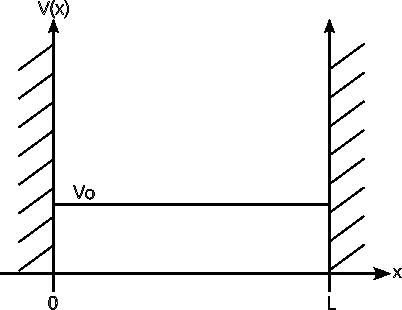
\includegraphics[width=0.5\textwidth]{../Figures/path469.pdf}
\end{figure}
Using Equation \ref{eq:1} we can write the perturbated hamiltonian for the infinite square well as 
\begin{align}
	\tilde{H} & = \hat{H}_0 + \lambda \hat{V}\nonumber\\
	& = \frac{-\hbar^2}{2m}\frac{d^2}{dx^2} + V_0,\,\,\,x \in\,\text[0,L]
\end{align}

So we have the Schr\"odinger equation
\begin{equation*}
	\frac{-\hbar^2}{2m}\frac{d^2 \tilde{\psi}_n(x)}{dx^2} + \lambda \tilde{V}_o \tilde{\psi}_n(x) 
	= \tilde{E}_n \tilde{\psi}_n(x)
\end{equation*}
for the perturbated system,
and the one for the unperturbated system
\begin{equation*}
	\hat{H}_o \psi_n = E_n \psi_n
\end{equation*}
so, we have a well known ODE
\begin{equation}
  \psi^{''}_n(x) = \frac{-2mE_n \psi_n(x)}{\hbar^2} 
\end{equation}
whose general solution is
\begin{equation}
 \psi_n (x) = A \cos\left( 
	\sqrt{\frac{2m E_n}{\hbar^2}}x\right) + B \sin\left( 
	\sqrt{\frac{2m E_n}{\hbar^2}}x\right) 
\end{equation}

Now, we need to apply the boundary conditions so we can find the constants $A$ and $B$
\begin{align*}
	\psi (0) & = \psi (L) = 0\\
	\psi(0) & = A \cancelto{1}{\cos(0)} + B \cancelto{0}{\sin(0)} + \Longrightarrow A = 0\\
	\psi(L) & = B \sin\left(\sqrt{\frac{2mE_n}{\hbar^2}L}\right) = 0 \Longrightarrow 
	\sqrt{\frac{2mE_n}{\hbar^2}L} = n\pi,\,\,\, n \in \mathbb{N}\,\,wlog
\end{align*}
therefore
\begin{equation*}
	E_n = \frac{n^2 \pi^2 \hbar^2}{2mL^2} \longleftarrow \text{Eigenenergies
		of the unperturbed infinite square well.}
\end{equation*}
\begin{equation}
  \label{eq:3.4}
	\psi(x) = B \sin \left(\frac{\sqrt{2m}}{\hbar}\left(\frac{n^2 \pi^2 \hbar^2}{2mL^2} \right)^{1/2}
	x\right) = B \sin \left(\frac{n\pi x}{L} \right)
\end{equation}

The Equation \ref{eq:3.4} is the wavefunction of the $n^{th}$ eigenstate of the infinite square well. But this wavefunction is not normalised, so we need to normalise it. 
\subsection{Normalisation}

To normalise the wavefunction we need to find the constant $B$ such that $\big<\psi_n\big|\psi_n\big> = 1$.
\begin{align}
	\big<\psi_n\big|\psi_n \big> & = 1 \nonumber\\
	& = B^2 \int_{0}^{L}\sin^2 \left(\frac{n\pi x}{L}\right)dx \nonumber \\
	& = B^2 \frac{L}{2} = 1 \nonumber\\
	\Aboxed{ B & = \sqrt{\frac{2}{L}}}
\end{align}

Then, replacing $B$ in Equation \ref{eq:3.4} we get
\begin{align}
  \label{eq:3.6}
	\psi_n (x) & = \sqrt{\frac{2}{L}} \sin \left(\frac{n\pi x}{L} \right),\,\,\,E_n = \frac{n^2 \pi^2
	\hbar^2}{2mL^2}\nonumber\\
  \intertext{\qquad From our previous results we know that the first and second order corrections to the eigenenergy are given by the following equation}
		\hat{E}_n & = E_n + \big<\psi_n\big|\hat{V}\big|\psi_n\big> + \sum_{n'\neq n} 
		\frac{\big|\big<\psi_{n'}\big|\hat{V}\big|\psi_n\big>\big|^2}{E_n - E_{n'}}
\end{align}

Substituting the results for $\psi_n$ and $E_n$  into Equation \ref{eq:3.6} we get 
\begin{equation*}
	\tilde{E}_n = \frac{n^2 \pi^2 \hbar^2}{2mL^2} +\int_{0}^{L} \frac{2}{L} \cancelto{1}{\sin^2 
		\left(\frac{n \pi x}{L} \right)}.V_0 dx + \sum_{n\neq n'} \frac{\bigg|\cancelto{0}{\int_{0}^{L} \sin 
	\left(\frac{n\pi x}{L}\right)} \sin \left(\frac{n, \pi x}{L}\right)dx \bigg|^2}{n^2 - n'^2} V^2_0 
	\frac{2m L^2}{\pi^2 \hbar^2}
\end{equation*}
\begin{equation}
  \label{eq:3.7}
	\boxed{\tilde{E}_n  = \frac{n^2 \pi^2 \hbar^2}{2mL} + V_0 }
\end{equation}

Basically, if we add a constant potential $V_0$ everywhere, this just shifts the eigenenergies 
by $V_0$. \\

The $2^{nd}$ order term is zero because $V_0$ does not alter the wavefunction $\psi_n$ and 
$\big<\psi_{n'}\big|\psi_n \big > = \delta_{n'n}$.

Now, let's consider the case for a perturbative potential $V_0/2$.
If we half the potential, the eigenenergies will be shifted by $V_0/2$
\begin{multline*}
	E_n = \frac{n^2 \pi^2 \hbar^2}{2mL} + \int_{0}^{\frac{L}{2}} V_0 \sin^2 \left(\frac{n\pi x}
	{L}\right)\frac{2}{L} dx\\
	+ \sum_{n\neq n'} \frac{V^2_0}{n^2 - n'^2} \frac{2mL^2}{\pi^2 \hbar^2}\bigg|\int_{0}^{\frac{L}{2}}
	\sin\left(\frac{n\pi x}{L}\right)\sin\left(\frac{n'\pi x}{L}\right)dx \bigg|^2
	\left(\frac{2}{L}\right)^2
\end{multline*}
\begin{multline*}
	E_n = \frac{n^2 \pi^2 \hbar^2}{2mL} +V_0 \frac{2}{L} \left(\frac{L}{2\cdot 2}\right) + \frac{2mL^2}
	{\pi^2 \hbar^2}V_0^2 \sum_{n'\neq n} \frac{1}{n^2 - n'^2}\cdot \bigg| \frac{1}{2}\int_{0}^
	{\frac{L}{2}} \cos \left(\frac{(n-n')\pi x}{L}\right)\\
	+ \cos \left(\frac{(n+n')\pi x}{L}\right)dx \bigg|^2\cdot \left(\frac{2}{L}\right)^2
\end{multline*}
\begin{multline*}
	E_n = \frac{n^2 \pi^2 \hbar^2}{2mL} + \frac{V_0}{2} + \frac{2mL^2 V^2_0}{\pi^2 \hbar^2}\sum_{n'\neq n}
	\frac{1}{n^2 - n'^2}\frac{1}{4}\cdot \Bigg|\frac{L}{\pi}\left(\frac{\sin\left(\frac{(n-n')x\pi}{L}\right)}
	{n-n'}\right)\\
	-\left(\frac{\sin\left(\frac{(n+n')x\pi}{L}\right)}{n+n'}\right)\Bigg|_{0}^{\frac{L}{2}}\Bigg|^2
\left(\frac{2}{L}\right)^2
\end{multline*}
\begin{equation*}
 E_n = \frac{n^2 \pi^2 \hbar^2}{2mL} + \frac{V_0}{2} + \frac{2mL^2 V^2_0}{\pi^2 \hbar^2}\sum_{n'\neq n}
 \frac{1}{n^2-n'^2}\Bigg|\frac{\sin((n-n')\pi/2)}{n-n'} +\frac{\sin((n+n')\pi/2)}{n+n'}\Bigg|^2
\end{equation*}
\begin{multline*}
 E_n = \frac{n^2 \pi^2 \hbar^2}{2mL} +\frac{V_0}{2} + \frac{2mL^2 V^2_0}{\pi^2 \hbar^2}\sum_{n'\neq n}
 \frac{1}{(n-n')(n+n')}\Bigg|\frac{(1-(-1)^{n-n'})}{2}\frac{(-1)^{\frac{n-n'-1}{2}}}{n-n'}\\
 + \frac{(1-(-1))^{n+n'}(-1)^{\frac{n+n'}{2}}}{n+n'} \Bigg|^2
\end{multline*}
\textbf{If $n+n,$ is even, then $n-n,$ is even.}\\
Proof:
\begin{align*}
	n+n' & = 2k\\
	n-n' & = n+n' -2n'=2k -2n'\,\,\Longrightarrow\text{Which is even.}
\end{align*}
\textbf{If $n+n,$ is odd, then $n-n,$ is odd.}\\
Proof:
\begin{align*}
	n+n' & = 2k + 1\\
	n-n' & = n+n'-2n' = 2k+1-2n'\\
	& = 2(k - n') + 1\,\,\Longrightarrow \text{is odd.}
\end{align*}
Then:
\begin{equation*}
	\frac{1-(-1)^{n-n'}}{2} = \frac{1-(-1)^{n+n'}}{2}
\end{equation*}
\begin{align*}
	\tilde{E}^{(2)}_n & = \frac{2mL^2V_o^2}{\pi^4 \hbar^2}\sum_{n'\neq n}\frac{1}{(n-n')(n+n')}\bigg|
	\frac{1-(-1)^{n+n'}}{2} \bigg|\bigg|\frac{(-1)^{\frac{n-n'-1}{2}}}{n-n'} + \frac{(-1)^{\frac{n+n'}
{2}}}{n+n'} \bigg|^2
\end{align*}
Only when $n+n'$ is odd we have a correction.
\begin{align*}
	\tilde{E}^{(2)}_n & = \frac{2mL^2V_o^2}{\pi^4 \hbar^2}\sum_{n'\neq n}\frac{1}{(n-n')(n+n')}\bigg|
	\frac{1-(-1)^{n+n'}}{2} \bigg|\bigg|(-1)^{\frac{n+n'}{2}}\bigg|^2\bigg|\frac{1}{n+n'} - 
	\frac{1}{n-n'}\bigg|^2\\
	& =\frac{2mL^2V_o^2}{\pi^4 \hbar^2}\sum_{n'\neq n}\frac{1}{(n-n')(n+n')}\left(
	\frac{1-(-1)^{n+n'}}{2}\right) \Bigg|\frac{n-n'-(n+n')}{(n+n')(n-n')}\Bigg|^2\\
	& = \frac{8mL^2V_o^2}{\pi^4 \hbar^2}\sum_{n'\neq n} \frac{n'^2}{(n^2 - n'^2)^3}\frac{1-(-1)^{n+n'}
	}{2}
\end{align*}
We only have a 2nd order correction when we go odd $\rightarrow$ even or even $\rightarrow$ odd.\\
\\
\textbf{Suppose n is even:}\\
\begin{align*}
	n = 2k \Longrightarrow \Psi_{2k}\left(\frac{L}{2}\right) & = 0\\
	\Psi_{2k + 1} \left(\frac{L}{2}\right) & = \pm \sqrt{\frac{2}{L}}
\end{align*}
%%%%%%%%%%%%%%%%%%%%%%%%%%%%%%%%%%%%%%%%%%%%%%%%%%%%%%%%%%%%%%%%%%%%%%%%%%%%%%%%%%%%%%%%%%%%%%%%%%
%%%%%%%%%%%%%%%%%%%%%%%%%%%%%%%%%%%%%%%%%%%%%%%%%%%%%%%%%%%%%%%%%%%%%%%%%%%%%%%%%%%%%%%%%%%%%%%%%%
%%%%%%%%%%%%%%%%%%%%%%%%%%%%%%%%%%%%%%%%%%%%%%%%%%%%%%%%%%%%%%%%%%%%%%%%%%%%%%%%%%%%%%%%%%%%%%%%%%
\subsection{Example 3.3}
Let's consider the infinite square well potential with a perturbative potential $V(x) = \alpha \delta(x-\frac{L}{2})$.
\begin{figure}[h]
  \centering
	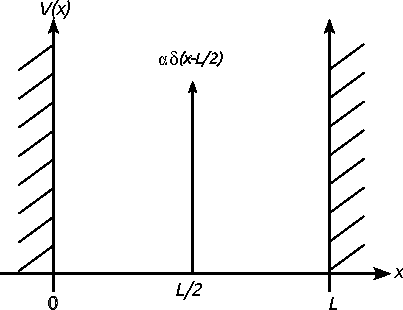
\includegraphics[width=0.5\textwidth]{../Figures/delta.pdf}
\end{figure}
From the aforementioned results we can state the criteria for using perturbation theory:
\begin{equation*}
  \boxed{\big|\big<\psi_{n'}\big|\hat{V}\big|\psi_n\big>\big|^2 \ll (E_n - E_{n'})^2}
\end{equation*}
\begin{equation*}
  \boxed{ \psi_n = \sqrt{\frac{2}{L}} \sin \left(\frac{n\pi x}{L}\right),\,\,\,\,\,\,\,\,\,\,\,\,\,\,\,\,
  E_n = \frac{n^2 \pi^2 \hbar^2}{2mL^2}}
\end{equation*}
\begin{align*}
	\big|\big<\psi_{n'}\big|\hat{V}\big|\psi_n\big>\big|^2 & = \Bigg |\alpha\int_{0}^{L}\frac{2}{L}
	\sin\left(\frac{n'\pi x}{L}\right) 	\sin\left(\frac{n\pi x}{L}\right) \delta \left(x - 
	\frac{L}{2}\right)dx\Bigg|^2\\
	& = \frac{4}{L^2}\alpha^2 	\sin^2\left(\frac{n'\pi}{L}\right)\sin^2\left(\frac{n\pi}{L}\right)\\
	& = \left(\frac{2\alpha}{L}\right)^2 \underbrace{\left(\frac{1-(-1)^{n'}}{2}\right)}_\text{n' is
	odd}\underbrace{\left(\frac{1-(-1)^{n}}{2}\right)}_\text{n is odd}
\end{align*}
\begin{equation*}
	(E_n-E_{n'})^2 = \left(\frac{\pi^2 \hbar^2}{2mL^2}\right)(n^2 - n'^2)^2
\end{equation*}
\begin{equation*}
	\frac{4\alpha^2}{L^2} \ll \frac{\pi^4 \hbar^4}{4m^2L^4}(n-n')^2(n+n')^2
\end{equation*}
\begin{equation*}
	\alpha \ll \frac{\pi^2 \hbar^2}{2mL}\big|n^2 - n'^2\big| = \frac{\pi^2 - n'^2}{2mL}
	\underbrace{(n-n')}_{\geq 2}\underbrace{(n+n')}_{\geq 4}
\end{equation*}
\begin{equation*}
	\alpha << \frac{4 \pi^2 \hbar^2}{mL}
\end{equation*}
\begin{align*}
	\tilde{E}^{(1)}_n & = \big<\psi_n \big| \hat{V}\big|\psi_{n}\big>\\
	& = \int_{2}^{L} \frac{2}{L} \sin^2 \left(\frac{n\pi x}{L}\right)\alpha\delta\left(x - \frac{L}{2}
	\right)dx\\
	& = \frac{2}{L}\sin^2 \left(\frac{n\pi L}{2L}\right)\cdot \alpha \cancelto{0}{\int_{0}^{L}
	\delta\left(x - \frac{L}{2}\right)}\\
	& = \frac{2}{L}\left(\frac{1-(-1)^n}{2}\right)
\end{align*}
\begin{equation*}
	\tilde{E}_{2k} = \frac{\pi^2 \hbar^2 (2k)^2}{2mL^2} + 0
\end{equation*}
when $\psi_{2k}$ has no $1^{st}$ order correction to their eigenenergies.
\begin{equation*}
	\tilde{E}_{2k-1} = \frac{\pi^2 \hbar^2 (2k-1)^2}{2mL^2} + \frac{2\alpha}{L}
\end{equation*}
odd $\psi_{2k-1}$ have a constant shift by $\frac{2}{L}\alpha$.
\begin{equation*}
	\psi_{2k}\left(\frac{L}{2}\right) = \sqrt{\frac{2}{L}} \sin\left(\frac{2k\pi L}{2L}\right) = 
	\sqrt{\frac{2}{L}}\sin(\pi k)= 0
\end{equation*}
even $n$ index wavefunctions all have a node @ $\frac{L}{2}\rightarrow \left(
\psi_{2k}\left(\frac{L}{2}\right)=0\right)$.\\
\\
Since $V(x) = \alpha \delta\left(x - \frac{2}{L}\right)$ is non-zero only @ $\frac{L}{2}$ it does nothing to the even
n wavefunctions.\\
\\
$\because$ a particle in the $2k-1$, odd n, state $\psi_{2k-1}$ has a probability $\Big|\psi_{2k-1}
\left(\frac{L}{2}\right)\Big|^2 = \frac{2}{L}$ of being @ $\frac{L}{2}$.
\newpage























\end{document}
